\subsection{File characterization}

\paragraph{File type}

\begin{figure*}
	\centering
	\includegraphics[width=1\textwidth]{graphs/graph-types-hierarchy}
	\caption{Taxonomy of file types.
	}
	\label{fig:file-type-hierarchy}
\end{figure*}

In this section, we present our redundant file characterization on file repeat count, file size, and file types. 
Based on this characterization, we create three-level classification hierarchy as shown in Figure~\ref{fig:file-type-hierarchy}.
At the highest level, we created two categories: \textit{High redundant file types and low redundant file types} based on the total redundant file size for each type. 
Totally, we got around 1,500 types after analyzing our whole dataset. 
We found that only 133 file types's total redundant file sizes are greater than 5 GB, which take up to 98.4\% files with 166.8 TB totally. We put these 133 file types into high redundant file type group and the remaining files into low redundant file types. Our further classification expands on the 98.4\% common redundant file types. 
%
%are common file types that consists of a largest number of redundant files with large storage space consumed, such as xxx and xxx. 
%Only xxxx\% files are non-common file types that only contains a small number of redundant files with less storage space, such as xxxx and xxxx. 

At the second level of the hierarchy, we clustered high redundant file types based on the \textit{major file format, usage or platform} involved by each file type. We identified redundant files' types relevant to \textit{EOF (executable, object code, and libraries), source code, scripts, documents, archival, images, databases, and others}.

At the third level, we present the specific redundant file types which take a large percentage of redundant files or storage space.
% or further classify the redundant files based on involved by each file type. 
%We selected the file types which take largest storage space.  


%\subsection{File repeat count}
%\subsection{File size}

\paragraph{File size}

\begin{figure}
	\centering
	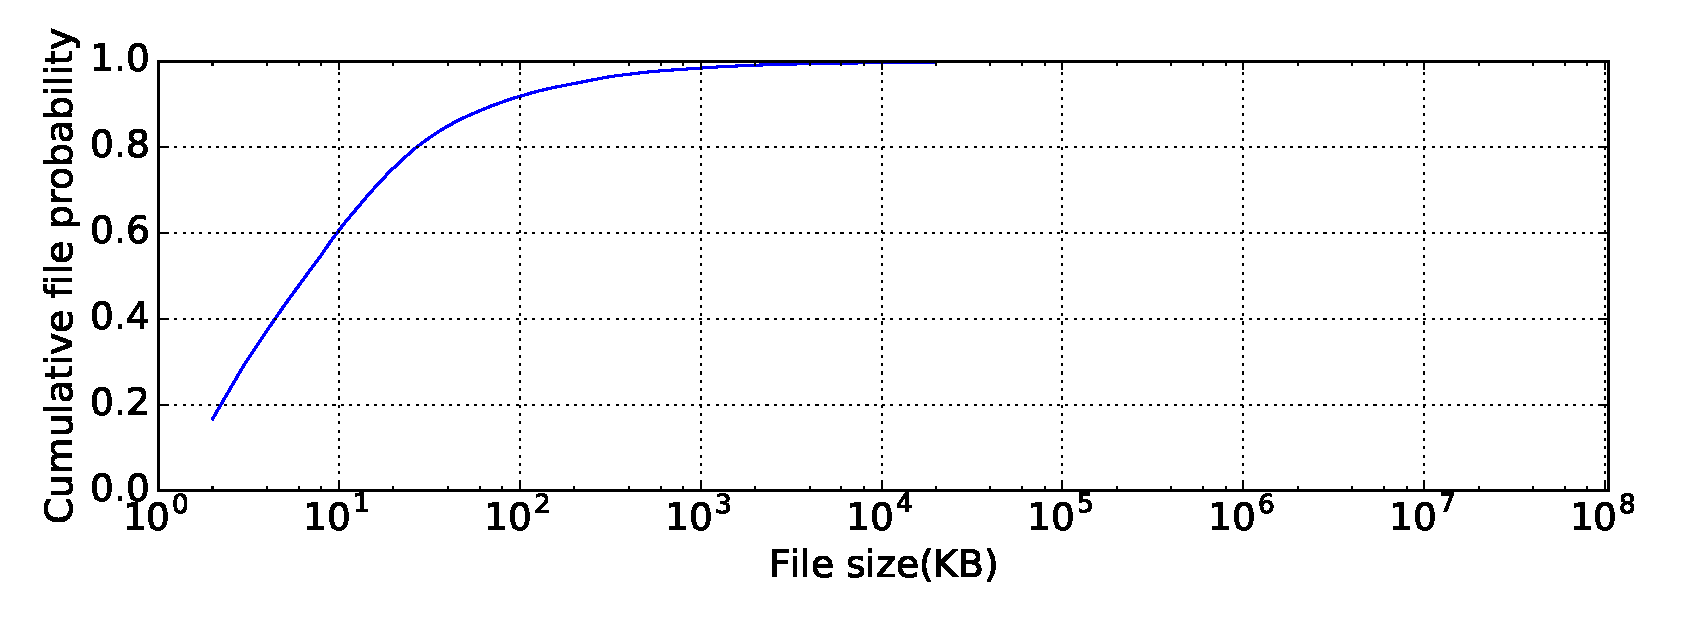
\includegraphics[width=0.5\textwidth]{graphs/File_size-KB.eps}
	\caption{File size distribution.
		}
		\label{fig:file-size}
		\end{figure}
		
		Figure~\ref{fig:file-size} shows the cumulative and probability distribution of file size.
		%of unique dataset after we remove the redundant files.
		\textit{Most files are smaller files.} For example, 91\% files'sizes are equal or less than 100KB. 
		Around 22\% of files are less than 1 KB.


\paragraph{File repeat count}
\begin{figure}
	\centering
	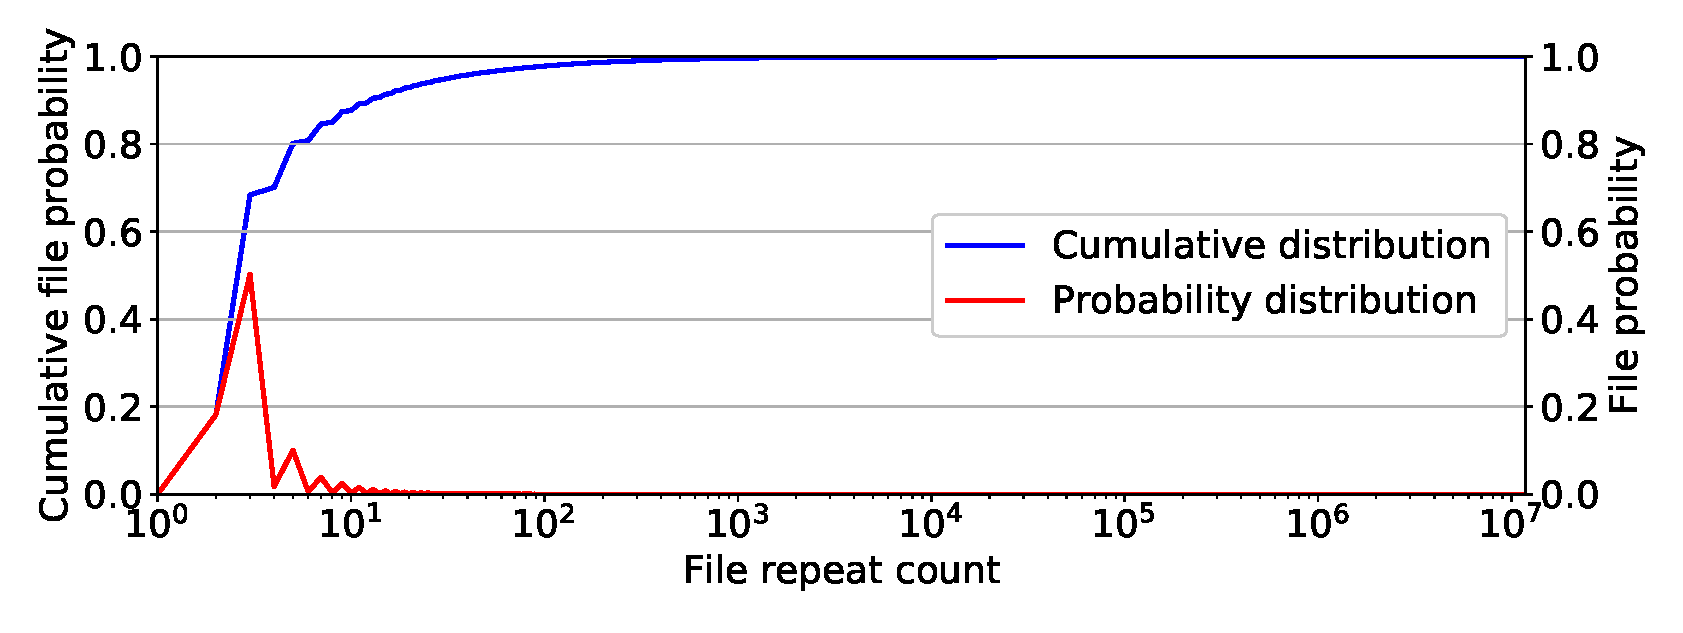
\includegraphics[width=0.5\textwidth]{graphs/File_repeat_count.eps}
	\caption{File repeat count distribution.
	}
	\label{fig:file-repeat-cnt}
\end{figure}

Figure~\ref{fig:file-repeat-cnt} shows the cumulative and probability distribution of file repeat count. 
Most files have a small repeat count. For instance, almost 90\% of files have equal or less than 10 copies. Around 50\% of files have 4 copies.
The file that has the maximum repeat count is empty file, which means that many users creates empty files and stored in their images.
%As shown in Table~\ref{fig_image_growth}, the number of repositories increased
%linearly during our observation period from May 30th to September 20th,
%2017. Note that the graph shows a gap of 15 days due to Docker Hub changing the way it
%indexes repositories. The total number of repositories
%grew from 633,915 to 687,292, resulting in an average creation rate of 1,241
%repositories per day.
%This rapid growth of repositories suggests that storage optimizations will
%be crucial for registries in the neear future.
%Notice also,
%that each repository contains multiple tagged images and, therefore, we 
%significantly underestimatet the size of Docker Hub's content.